
% This LaTeX was auto-generated from MATLAB code.
% To make changes, update the MATLAB code and republish this document.

\documentclass{article}
\usepackage{graphicx}
\usepackage{color}
\usepackage{amsmath}
\usepackage{amssymb}
\usepackage[a4paper, total={6in,8in}]{geometry}
\usepackage{pdfpages}
\usepackage{multicol}

\sloppy
\definecolor{lightgray}{gray}{0.5}
\setlength{\parindent}{0pt}

\begin{document}


\includepdf{../TitlePage.pdf}

\hrulefill
\subsection*{\#1}

\begin{verbatim}
clear;clc;close all
[x, y] = meshgrid(linspace(0,5,100),linspace(0,pi(),100));
len = size(x);
for i = 1:len(1)
    for j = 1:len(2)
        f = @(n) exp(-(2.*n-1).*x(i,j)).*sin((2.*n-1).*y(i,j))./(2.*n-1);
        T(i,j) = 4/pi()*limsum(f);
    end
end
figure()
surf(x,y,T)

f = @(n) 4/pi()*exp(-(2.*n-1).*1).*sin((2.*n-1).*(pi()/2))./(2.*n-1);
sum = 0;
n = 1;
while 1
    error = f(n);
    sum = sum + error;
    if abs(error) < 1e-6
        break
    end
    n = n+1;
end
fprintf("For T(1,pi/2): \n    Iteration times: %d \n    Value: %f \n    Error: %f\n\n", n, sum, error)

f = @(n) 4/pi()*exp(-(2.*n-1).*0.0369).*sin((2.*n-1).*(0.01*pi()))./(2.*n-1);
sum = 0;
n = 1;
while 1
    error = f(n);
    sum = sum + error;
    if abs(error) < 1e-6
        break
    end
    n = n+1;
end
fprintf("For T(0.0369,0.01pi): \n    Iteration times: %d \n    Value: %f \n    Error: %f\n\n", n, sum, error)

figure()
plot(x(1,:), T(1,:))
title("T(x,0)",'FontSize',15,'interpreter','latex')

figure()
plot(y(:,1), T(:,1))
title("T(0,y)",'FontSize',15,'interpreter','latex')
\end{verbatim}

\dotfill
\dotfill
        \color{lightgray} \begin{verbatim}For T(1,pi/2):
    Iteration times: 7
    Value: 0.448834
    Error: 0.000000

For T(0.0369,0.01pi):
    Iteration times: 98
    Value: 0.448859
    Error: -0.000001

\end{verbatim} \color{black}

\begin{multicols}{2}
    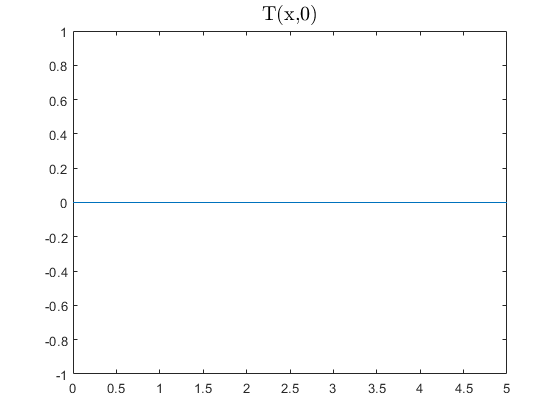
\includegraphics [width=3in]{HW2_02.png}
    \columnbreak
    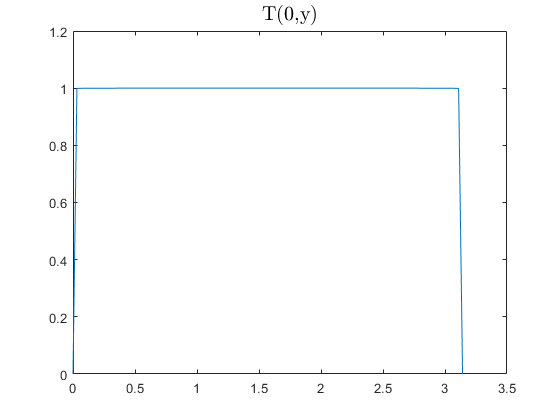
\includegraphics [width=3in]{HW2_03.png}
\end{multicols}


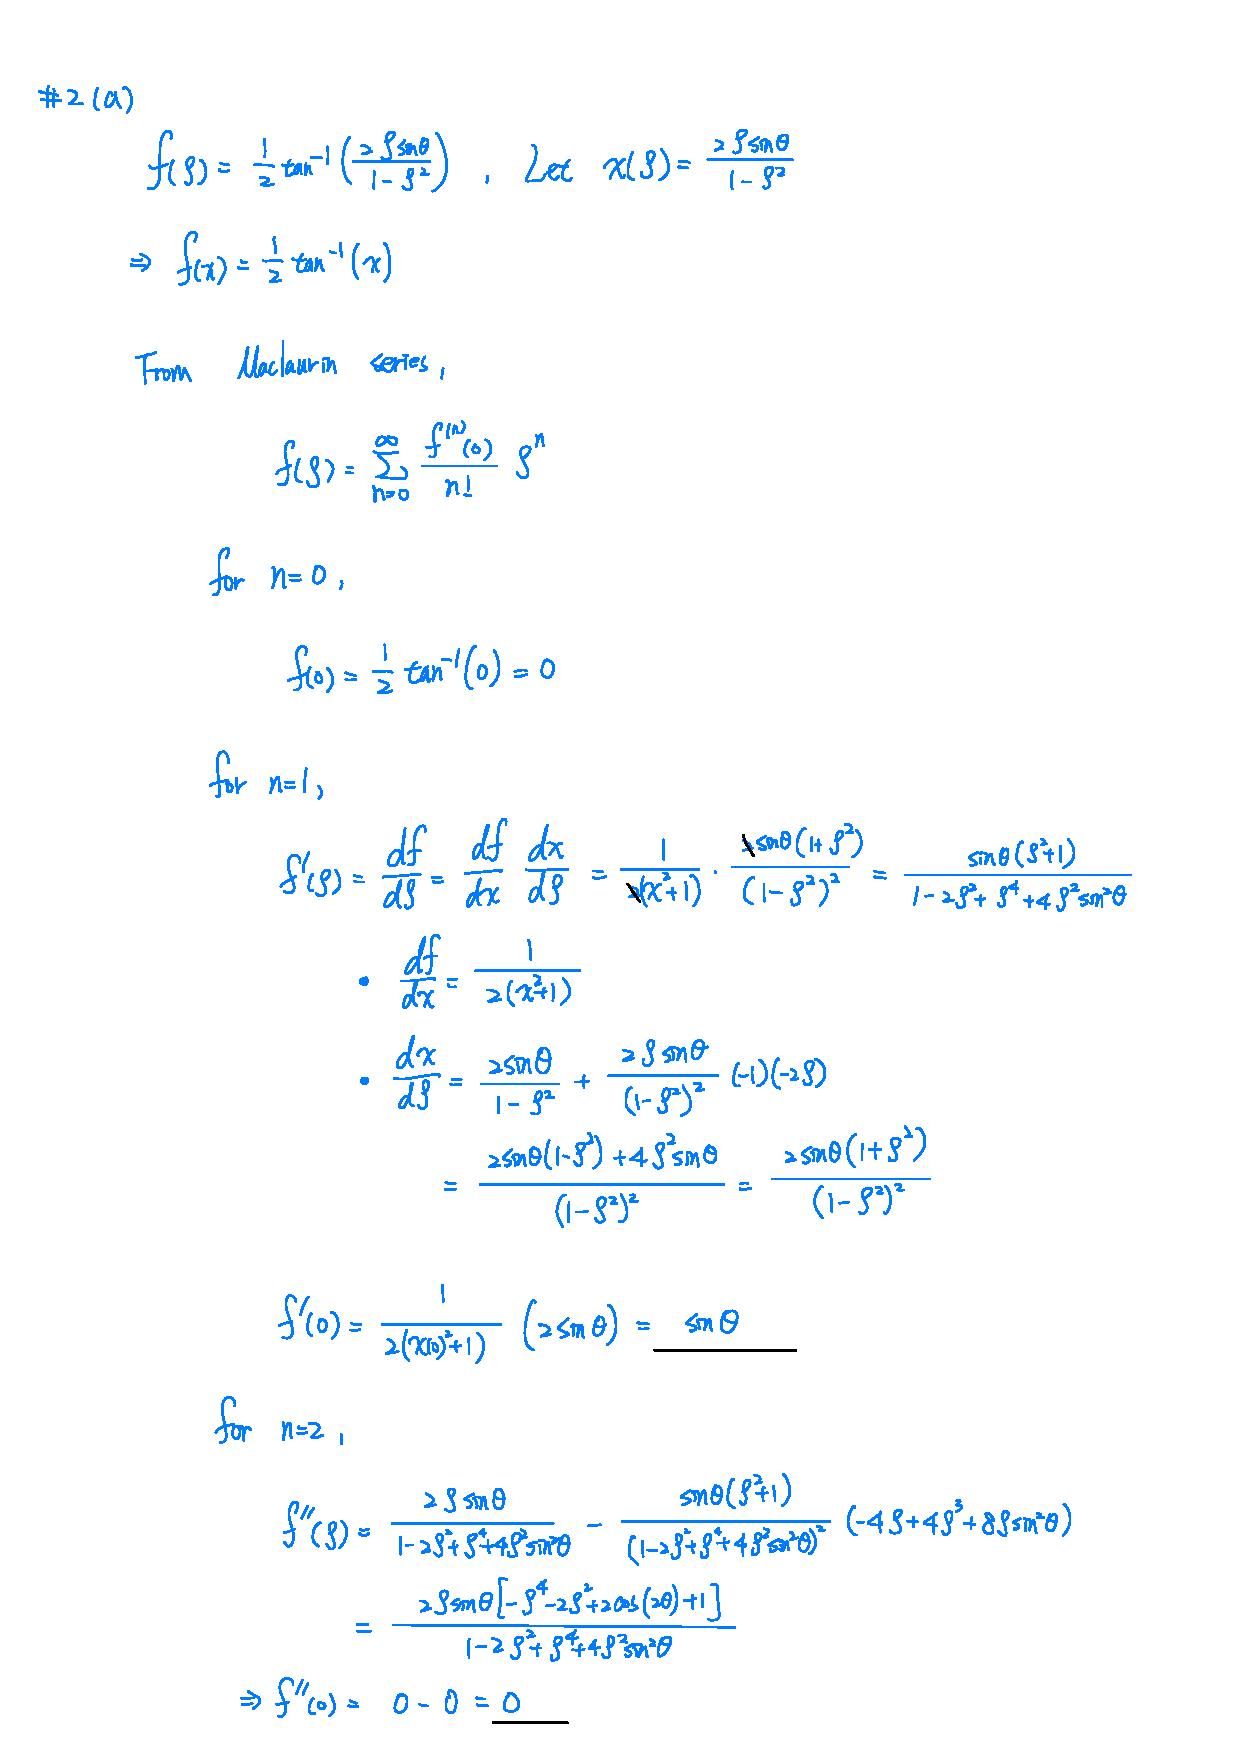
\includepdf[]{Q2_1.pdf}
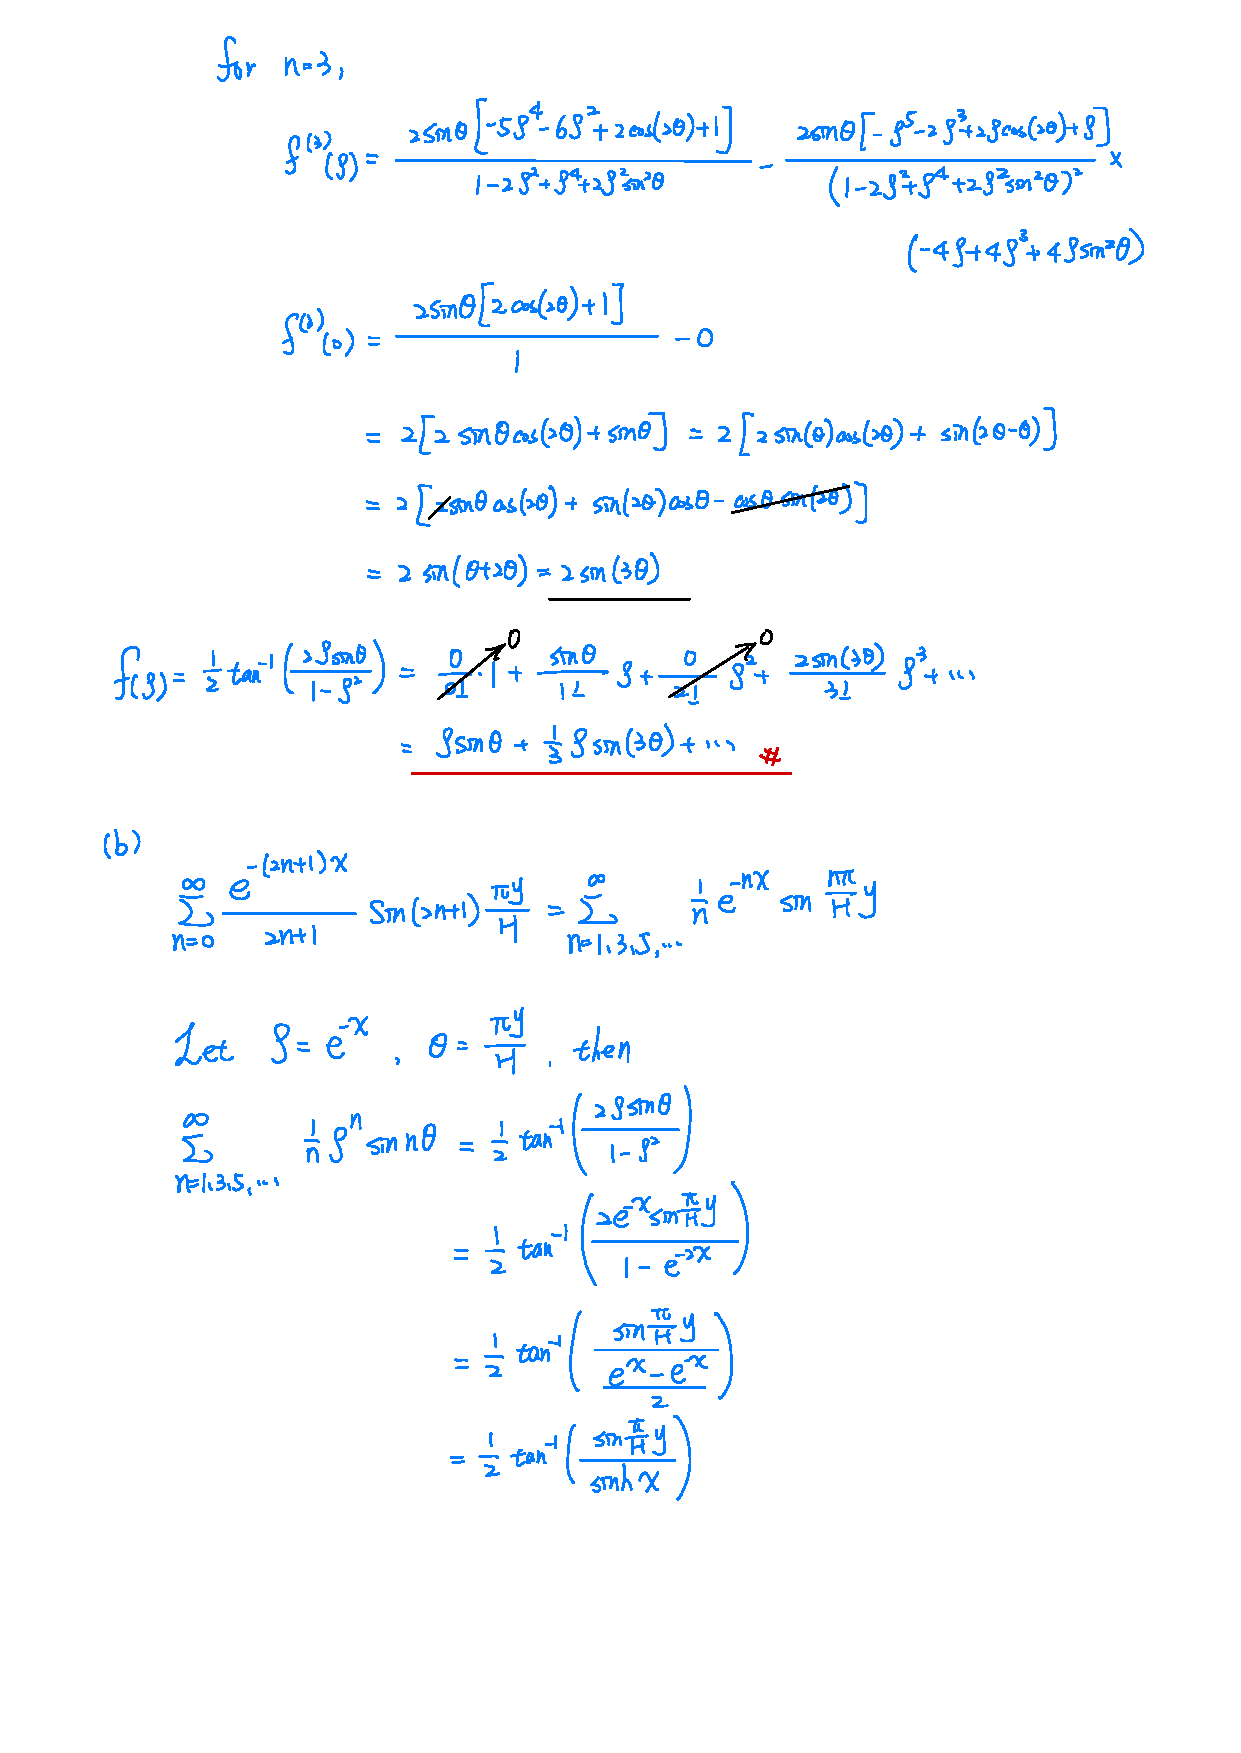
\includepdf[]{Q2_2.pdf}

\hrulefill
\subsection*{\#3}

\begin{verbatim}
clear;clc;close all
[x, y] = meshgrid(0:0.01:1,0:0.01:1);
len = size(x);
for i = 1:len(1)
    for j = 1:len(2)
        f = @(n) 2*exp(-n*pi().*y(i,j)).*sin(n*pi()/3).*sin(n*pi()*x(i,j));
        T(i,j) = limsum(f);
    end
end

figure()
surf(x,y,T, 'edgecolor', 'none')
title("$2\sum\limits^{\infty}_{n=1} e^{-n \pi y}\sin{\frac{n\pi}{3}}\sin{n \pi x}$ 3D Plot",'FontSize',15,'interpreter','latex')

figure()
plot(x(1,:), T(1,:))
% contour(x,y,T,'ShowText','on')
title("$2\sum\limits^{\infty}_{n=1} e^{-n \pi y}\sin{\frac{n\pi}{3}}\sin{n \pi x}$ 2D Plot",'FontSize',15,'interpreter','latex')

x = 0;
ended = 1;
step = 0.0001;
sum = 0;
while x<=ended
    f = @(n) 2*sin(n*pi()/3).*sin(n*pi()*x);
    sum = sum + limsum(f)*step;
    x = x+step;
end
fprintf("The answer of integral of T(x,0) from 0 to 1 is %.4f. \n", sum)
\end{verbatim}

\dotfill
        \color{lightgray} \begin{verbatim}The answer of integral of T(x,0) from 0 to 1 is 1.0000.
\end{verbatim} \color{black}

\newpage
\begin{multicols}{2}
    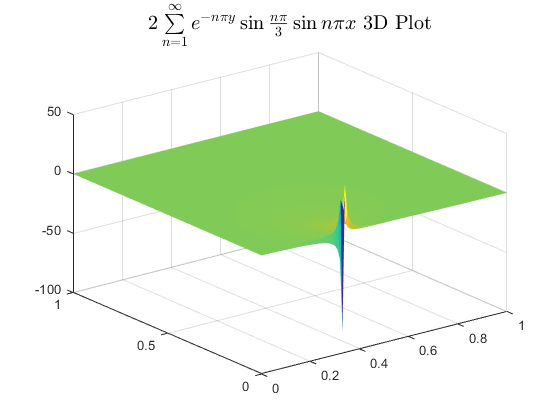
\includegraphics [width=3in]{HW2_04.png}
    \columnbreak
    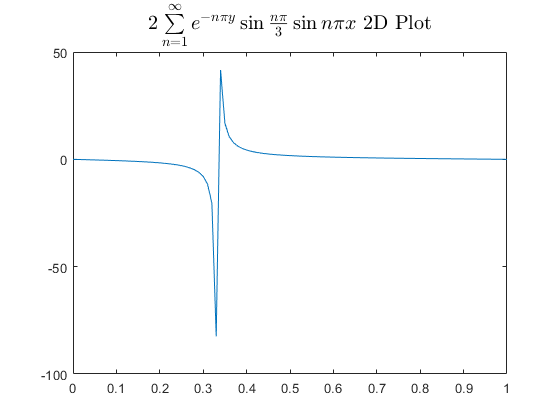
\includegraphics [width=3in]{HW2_05.png}
\end{multicols}


\hrulefill

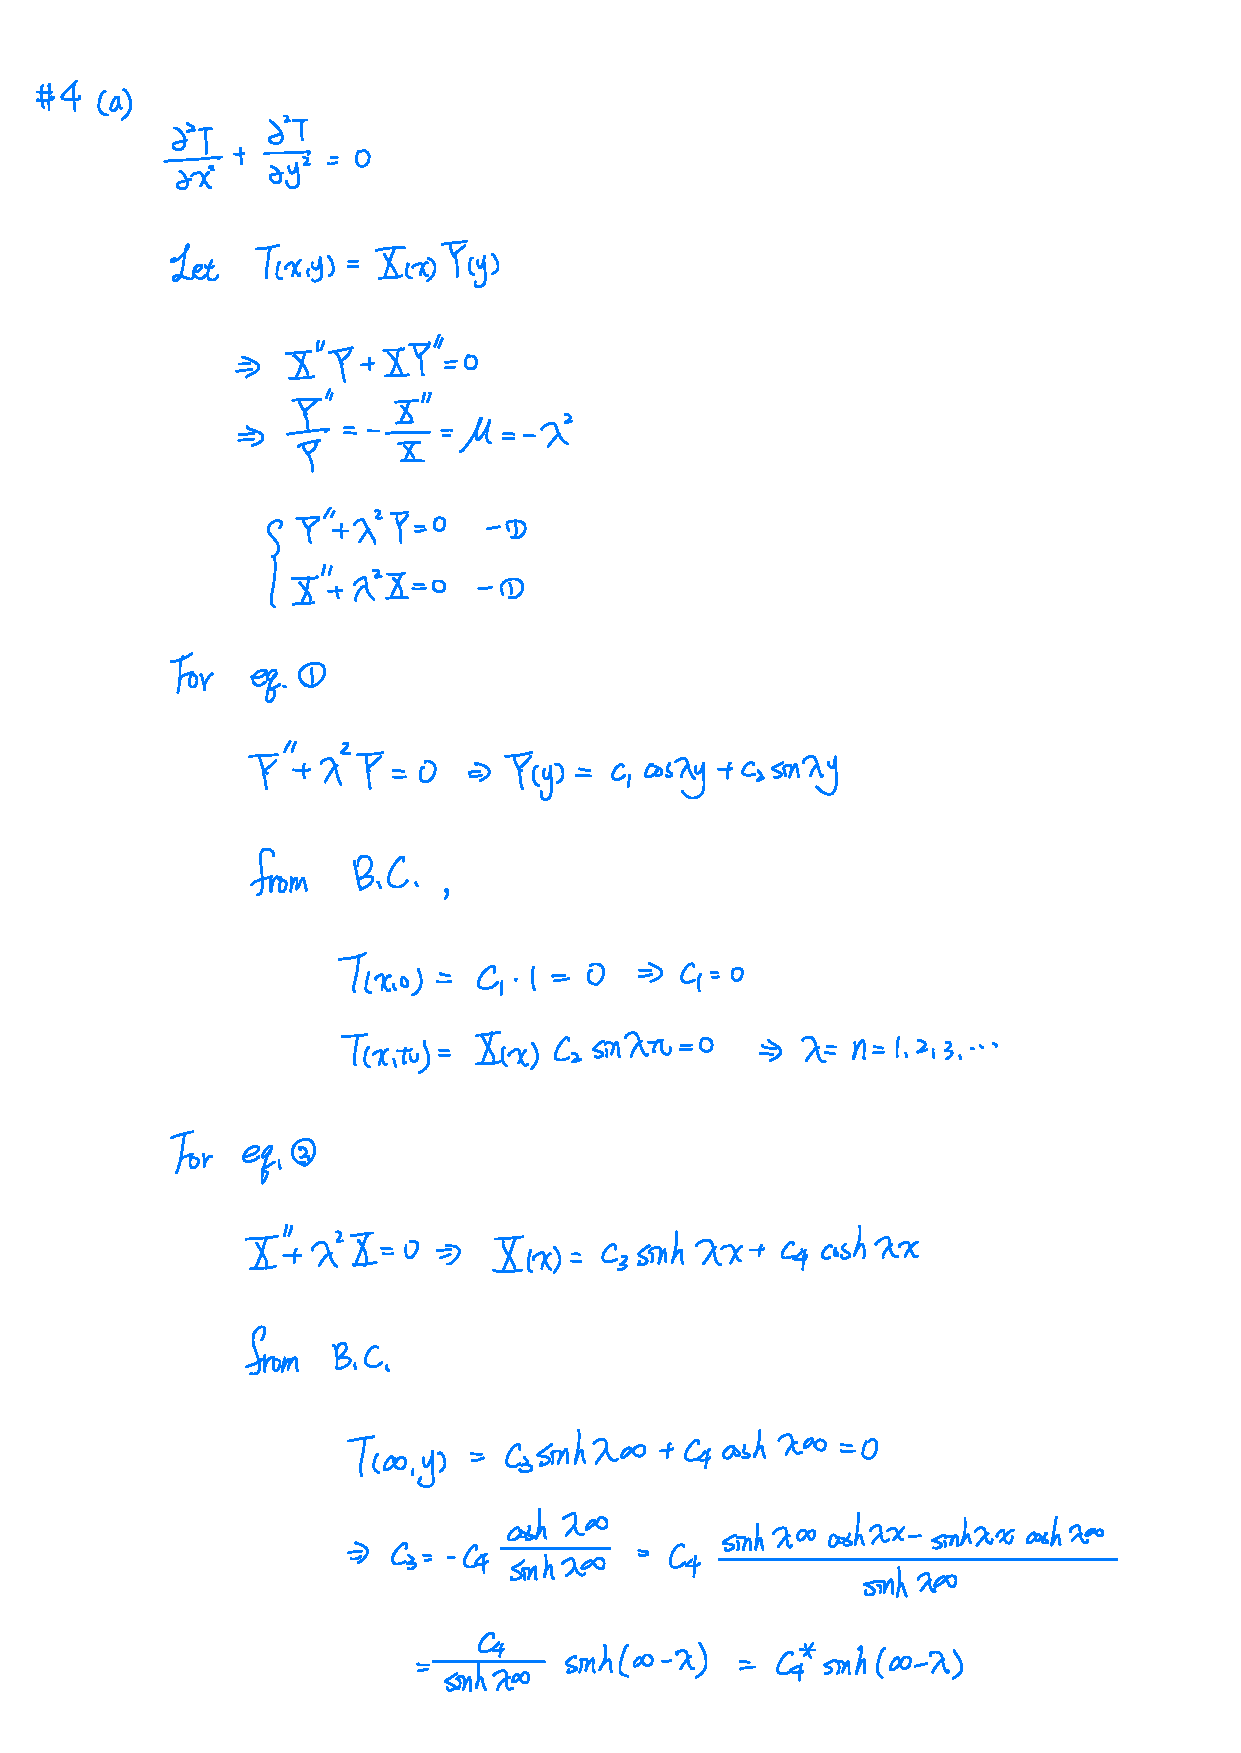
\includepdf[]{Q4.pdf}

\subsection*{\#4(b)}

\begin{verbatim}
clear;clc;close all

f = @(n) (4/pi).*(1./(2.*n-1)).*exp(-(2.*n-1).*0.88).*sin((2.*n-1).*pi/2);
sum = 0;
n = 1;
while 1
    error = f(n);
    sum = sum + error;
    if abs(error) < 1e-6
        break
    end
    n = n+1;
end
fprintf("For T0=1, then T(0.88,pi/2): \n    Iteration times: %d \n    Value: %f \n    Error: %f\n\n", n, sum, error)
\end{verbatim}

\dotfill
        \color{lightgray} \begin{verbatim}For T0=1, then T(0.88,pi/2):
    Iteration times: 8
    Value: 0.500619
    Error: -0.000000

\end{verbatim} \color{black}


\hrulefill
\subsection*{\#4(c)}

\begin{verbatim}
clear;clc;close all
T0 = 1;
x = 0.88;
y = pi()/2;
T = 2*T0/pi()*atan2(sin(y),sinh(x));
fprintf("T(0.88,pi/2) = %.4f\n", T)
\end{verbatim}

\dotfill
        \color{lightgray} \begin{verbatim}T(0.88,pi/2) = 0.5006
\end{verbatim} \color{black}


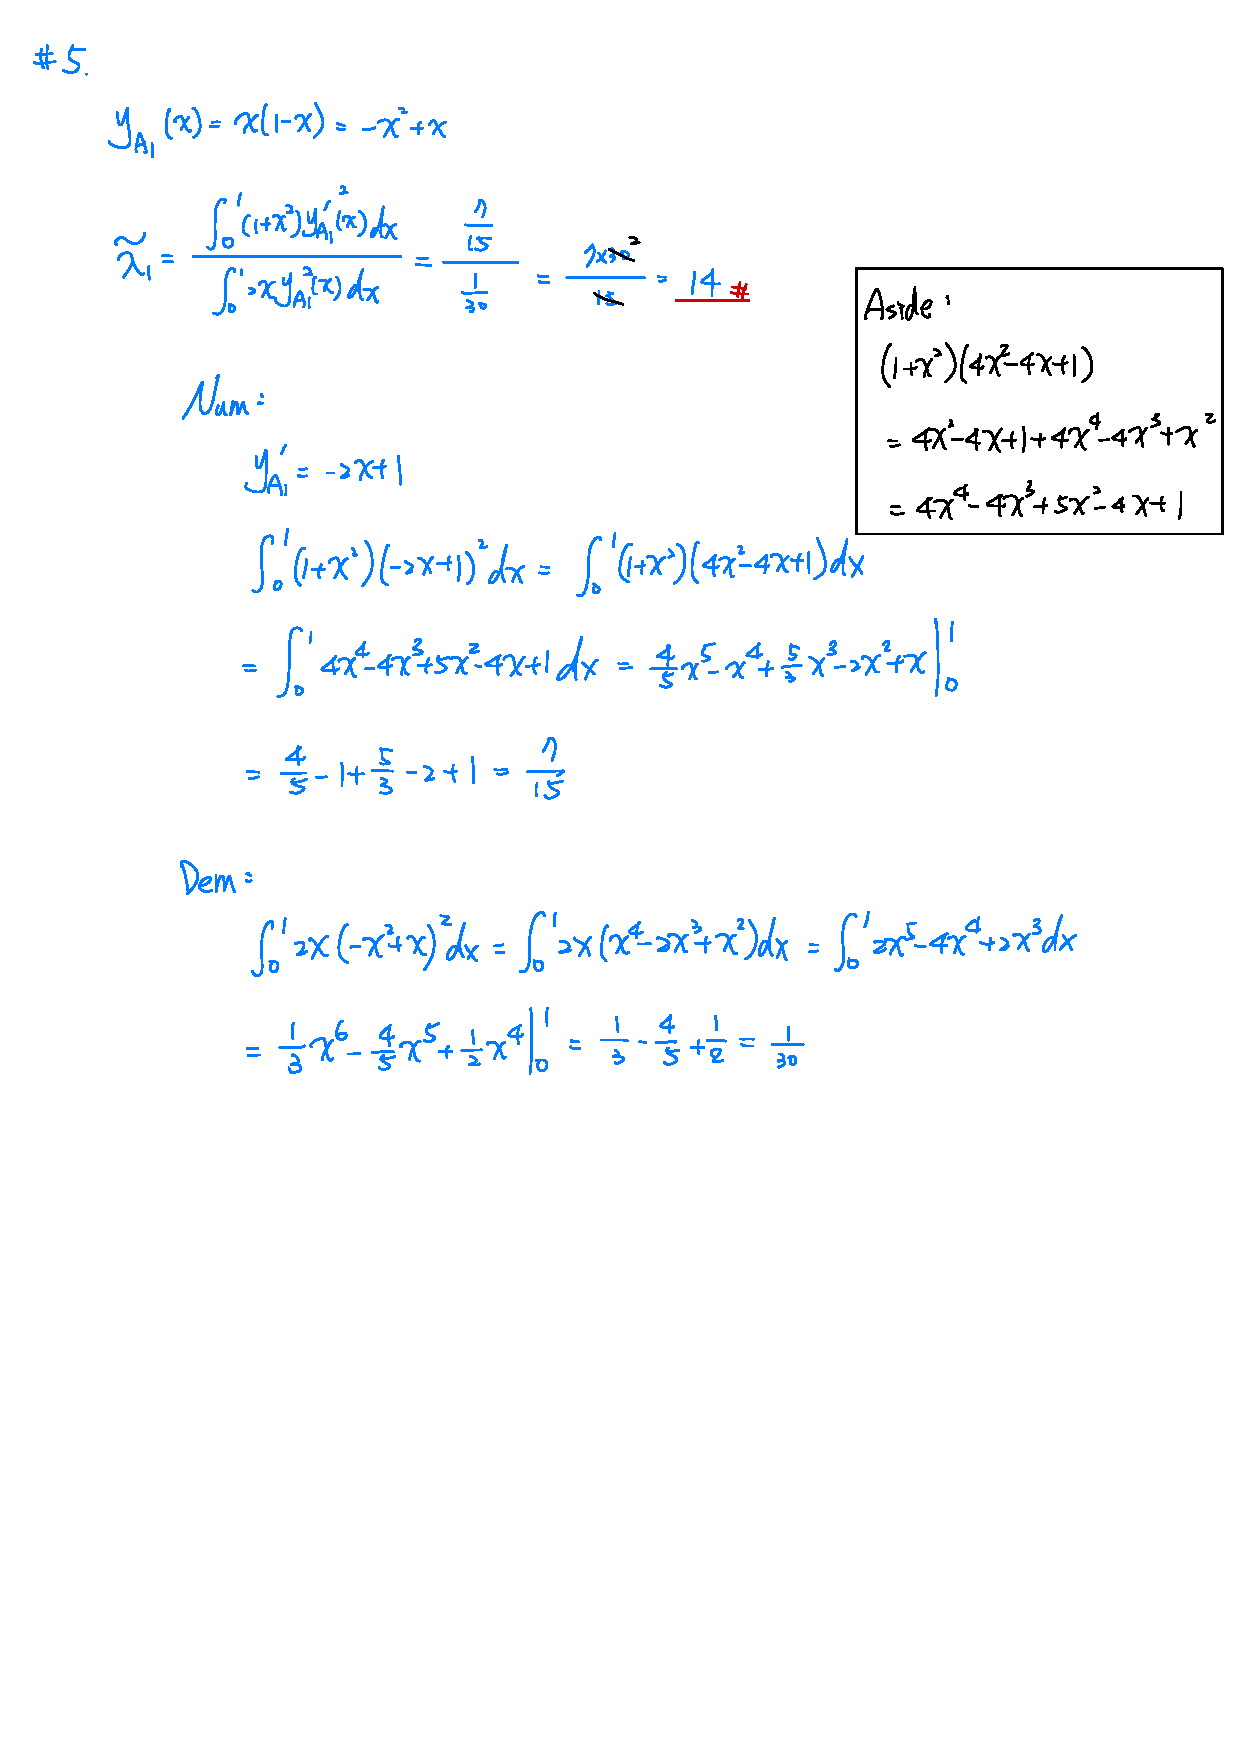
\includepdf[]{Q5.pdf}

\end{document}

